\section{Features to be tested}
\label{sec:GenerateChart}
\begin{figure}[h!] 
\centering 
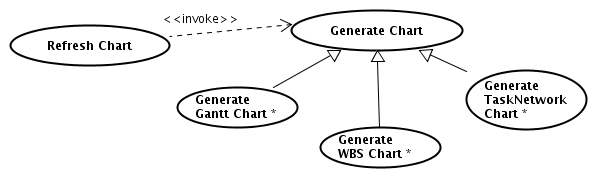
\includegraphics[width=0.7\textwidth]{desing_spec/GenerateChart.png}
\caption{spaccato tratto dal package \emph{Commons} del documento di analisi,
parte \emph{Use cases}}

\end{figure}
Verranno testati tutti gli use case espressi dalla figura tranne ``Refresh
Chart'' in quanto \`e stato riportato solo per favorire la comprensione del
contesto e perche la sua attivit\`a di costruire la \emph{UserOptionChoice} e
recuperare l'insieme dei \emph{Task} vengono testate nel documento
\footnote{make a test document for these use cases.}

\section{Raffinamento della strategia}
\begin{description}
  \item[confronto dell'output] Per ogni use case di ``generazione'' si
  fa riferimento alle notazioni espresse nel documento di specifica e se
  il budget del progetto lo consente, verranno prodotti dei modelli, in
  notazione \emph{mockup} disegnati a mano, per poter effettuare il confronto 
  con le immagini di output generate dall'implementazione.
  \item[modalit\`a di esecuzione] Ogni use case verr\`a esercitato in modo 
  \emph{individuale}, non verranno esercitate combinazioni con altri use case,
  come la figura esprime.
\end{description}

\section{Tests identification}
\label{sec:GenerateChartTestIdentification}
Sotto vi sono i reference a tutte le \emph{case specification} relative a
questo \emph{desing}, definite in \ref{part:CaseSpecification}:
\begin{itemize}
  \item \nameref{chap:generateGantt}
  \item \nameref{chap:generateWBS}
  \item \nameref{chap:generateTaskNetwork}
\end{itemize}

\section{Pass/fail criteria}
Il risultato di questo desing \`e
espresso dalla seguente relazione rappresentata da questa tabella: 
\begin{table}[h!]
  \begin{center}
    \begin{tabular}{| l | l |}
    \hline
    \textbf{risultato} & \textbf{criteri} \\
	\hline    
	success & numero di \emph{minor} failures $\leq 5$   \\
    \hline
    \emph{minor} failure & numero di \emph{minor} failures $> 5$ \\
    \hline
    \emph{critical} failure & almeno una \emph{critical} failure \\
    \hline
    \emph{blocking} failure & almeno una \emph{blocking} failure \\
    \hline
    \end{tabular}
  \end{center}
	\caption{La colonna \emph{criteri} si riferisce all'insieme di tests 
	identificati nella sezione \ref{sec:GenerateChartTestIdentification}}
\end{table}
